The following describes the hardware connected to the inverted pendulum setup illustrated cf. figure \ref{fig:InvertedPendulumSetUp}.
Each part will be described with its specifications and use in the setup. The input and output relation of each block is illustrated cf. figure \ref{fig:DCMotorRelation}, where the goal troughout the chapter will be determining the transfer functions that describe these relations.

\begin{figure} [htbp]
\hspace*{-3.5cm}  
	\centering
	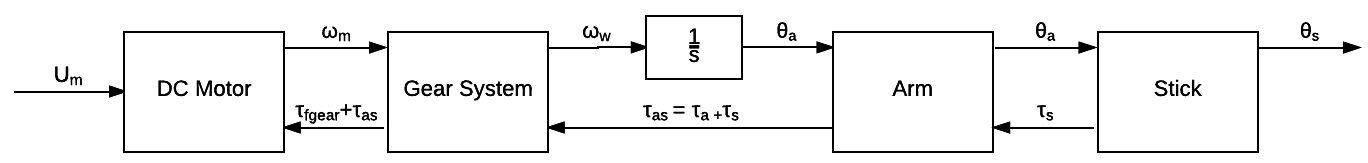
\includegraphics[width=0.95\paperwidth]{figures/modeling/InputOutputSystem.png}
	\caption{Input/output relation of the system plant.} \label{fig:DCMotorRelation}
\end{figure}

\startexplain
	\explain{$U_m$ is the motor input voltage}{\si{V}}
	\explain{$\omega_m$ is the angular velocity of the motor}{\si{\radian\per\second}}
	\explain{$\omega_w$ is the angular velocity of the gear connected to the arm}{\si{\radian\per\second}}
	\explain{$\tau_{f_{gear}}$ is the total friction of the gear system}{\si{\newton\meter}}
	\explain{$\tau_a$ is the load of the arm}{\si{\newton\meter}}
	\explain{$\tau_s$ is the load of the stick}{\si{\newton\meter}}
	\explain{$\theta_a$ is the angle from the arm to the y-axis}{\si{\radian}}
	\explain{$\theta_s$ is the angle from the stick to the y-axis}{\si{\radian}}
\stopexplain

\subsubsection{DC Motor}
A Axem DC servo motor model F9M2 is attached to the gears, this is to create a angular velocity in the system. To ensure control precision, the integrated tachometer of the motor is used as feedback. This is done so that it is possible to see the velocity and direction of the motor and relate it to the position of the arm. Using the DC motor also means implementing a motor controller. Already implemented in the setup is a Maxon Escon 50/5 Servocontroller, which can be controlled trough PWM. The servocontroller is supplied trough a 230 V regulator that can supply the servocontroller with up to 56 V and 15 A. The regulator in itself will be considered a blackbox, because of user limitations when working with 230 V at the university. The DC motor and servocontroller will in system diagrams be evaluated as one unit, but further considered when implementing a system controller.        

%http://www.maxonmotor.com/maxon/view/product/control/4-Q-Servokontroller/409510
	

\subsubsection{Gear System}
Inbetween the DC motor and arm is the gear system. The goal of the gear system is to reduce the ratio between the rotation of the motor versus the arm. The gear system is series of the same size small and big gear connected with belts. The setup is seen cf. figure \ref{fig:InvertedPendulumSetUp}, where the number of gear is illustrated. The parameters of the gear system is listed cf. table \ref{GearSystemParameters}.   

\begin{table}[htbp]
\centering
\begin{tabular}{llll}
\hline
Piece & Parameter & Value & Unit \\ \hline
Gear$_{big}$ & Teeth & 40 & {[}1{]} \\
Gear$_{big}$ & Diameter & 0.12 & {[}m{]} \\
Gear$_{small}$ & Teeth & 12 & {[}1{]} \\
Gear$_{small}$ & Diameter & 0.04 & {[}m{]} \\
Belt & Length & 0.6 & {[}m{]}
\end{tabular}
\caption{Parameters of gear system.}
\label{GearSystemParameters}
\end{table}

\subsubsection{Stick and Arm}
The arm and stick is elements that always appears in the double inverted pendulum setup. The goal is for the arm to apply force on their common joint, which would affect the position of the stick. The physical parameters for the stick and arm is listed cf. table \ref{DimensionsStick}.

\begin{table}[htbp]
\centering
\begin{tabular}{llll}
\hline
Piece           & Parameter & Value & Unit \\ \hline
Stick$_{long}$  & Length    & 0.8   & [m]    \\
Stick$_{long}$  & Weight    & 0.344 & [kg]    \\ 
Stick$_{short}$ & Length    & 0.4   & [m]    \\
Stick$_{short}$ & Weight    & 0.170 & [kg]    \\ 
Arm             & Length    & 0.33  & [m]    \\
Arm             & Weight    & 288   & [kg]   \\ 
\end{tabular}
\caption{Physical parameters of the arm and sticks.}
\label{DimensionsStick}
\end{table}
\newpage
Some feedback is needed to be able to control the stick trough the arm and gears. Sensors used is implemented as a integrated part of the setup, and will therefore be considered usable and will the choice of the will not be further discussed.

A necessary feedback to know is the angle between the stick and arm. This is needed to balance the stick via the controller. The angle between the stick and arm is detected and sampled from a potentiometers rotational position. Equally the position of the arm is needed, this is to determine the amount of change needed to counteract the change in the stick. The position of each potentiometer can be seen cf. figure \ref{fig:InvertedPendulumSetUpPotmeter}. 

\begin{figure} [htbp]
	\centering
	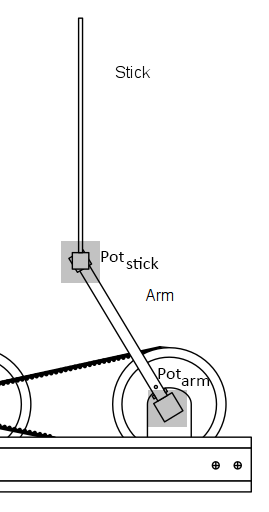
\includegraphics[width=0.35\linewidth]{figures/"Preanalysis&Requirement"/invertedPendulumWithPotmeter.png}
	\caption{Diagram of the arm and stick with illustrated sensors.} \label{fig:InvertedPendulumSetUpPotmeter}
\end{figure}
\newpage
The block diagram for the standard feedback control system with the known system plant is seen cf. figure \ref{fig:FeedbackSystem}. 

\begin{figure}[htbp]
\hspace*{-2.5 cm} 
	\centering
	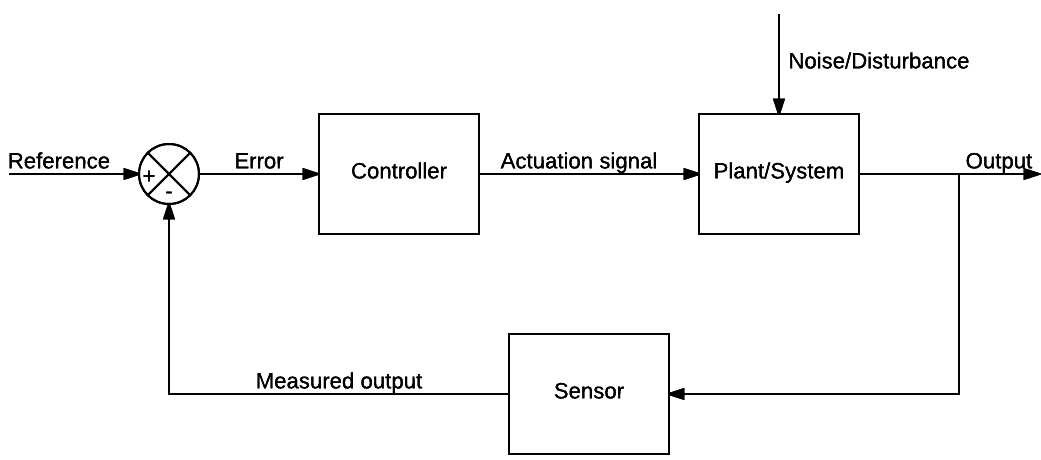
\includegraphics[width=0.95\paperwidth]{figures/modeling/MechanicalSystem.PNG}
	\caption{Setup feedback loop.} \label{fig:FeedbackSystem}
\end{figure}
\todo{Might be changed, was not sure how we would handle the feedback of the sensors.}
\\

The basics of each system in the Inverted Pendulum is now described with its specifications, and the dynamics of the system can therefore be modelled.


\newpage
